\subsubsection{Web Service}

    Du coté serveur, il faudra gérer plusieurs parties. D'un coté, il faut s'occuper des requêtes utilisateur, et de l'autre, il faut stocker certaines données que l'on renverra aux utilisateurs.

    Pour ce faire, l'architecture est la suivante.

    \begin{figure}[H]
        \centering
        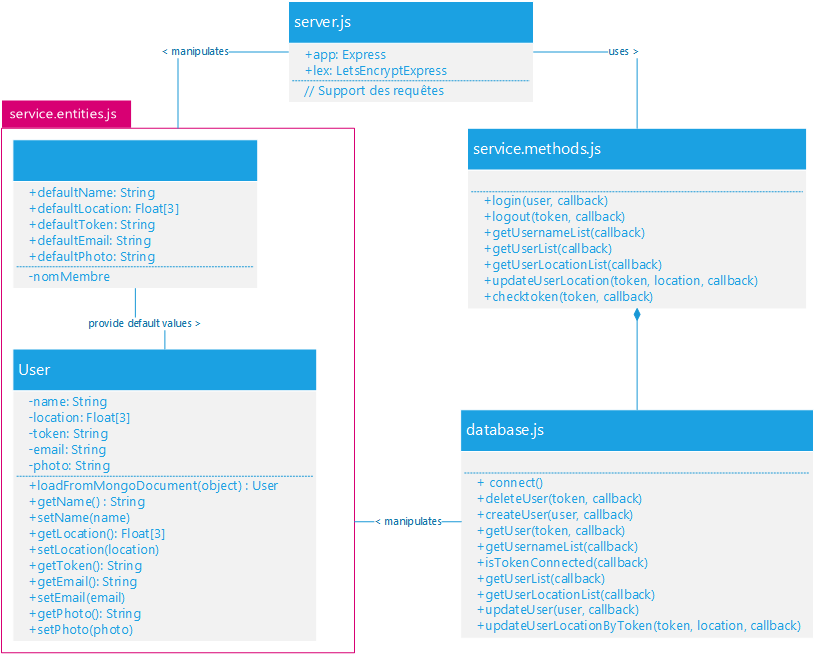
\includegraphics[width=\textwidth]{./img/architecture-service-web.png}
        \caption{Architecture du Service Web}
        \label{asweb}
    \end{figure}

    Comme nous pouvons l'observer dans la figure \ref{asweb}, blablabla.
    Le serveur + Mongodb.
    Pattern bridge pour la bdd. Des entités.